\documentclass{beamer}                             % presentation
\usepackage[utf8]{inputenc}                        % utf8
\usepackage[T1]{fontenc}                           % fix font encoding
\usepackage[english]{babel}                        % language
\usepackage[autostyle, english=american]{csquotes} % quotes
\usepackage{bm}                                    % extra math packages
\usepackage{graphicx, subcaption}                  % images
\usepackage{tikz, pgfplots}                        % plots and graphs
\usepackage[style=ieee]{biblatex}                  % bibliography
\usepackage{geometry, hyperref, enumitem}          % misc.

\usetikzlibrary{positioning}                       % advanced positioning
\pgfplotsset{compat=newest}                        % version of pgfplots

\graphicspath{{./figures/}}
\addbibresource{references.bib}

\renewcommand{\vec}[1]{\bm{#1}}

% serif font in math mode
\usefonttheme[onlymath]{serif}
% customize \item in itemize
\setitemize{label={},itemsep=0.5cm}

%%% colors

\definecolor{lightblue}{HTML}{a1b4c7}
\definecolor{orange}{HTML}{ea8810}
\definecolor{silver}{HTML}{b0aba8}
\definecolor{rust}{HTML}{b8420f}
\definecolor{seagreen}{HTML}{23553c}

\colorlet{lightsilver}{silver!20!white}
\colorlet{darkorange}{orange!85!black}
\colorlet{darksilver}{silver!85!black}
\colorlet{darklightblue}{lightblue!75!black}
\colorlet{darkrust}{rust!85!black}
\colorlet{darkseagreen}{seagreen!85!black}

\hypersetup{
  colorlinks=true,
  linkcolor=darkrust,
  citecolor=darkseagreen,
  urlcolor=darksilver
}

%%% beamer settings

\usetheme{Pittsburgh}
\usecolortheme{dolphin}

% hide navigation buttons
\setbeamertemplate{navigation symbols}{}
% change title color
\setbeamercolor{title}{fg=darklightblue}
\setbeamercolor{frametitle}{fg=darklightblue}
% change bibliography entry colors
\setbeamercolor{bibliography entry author}{fg=darklightblue}
\setbeamercolor{bibliography entry note}{fg=lightblue}

% title page
\title[]{Sparse Cholesky Factorization by \\ Greedy Conditional Selection}
\subtitle{}
\author[Huan, Sch{\"a}fer]
{Stephen Huan \and Florian\ Sch{\"a}fer}
\institute[Georgia Institute of Technology]
{
  Georgia Institute of Technology
}
\date[]{February 19, 2022}
\subject{Computer Science}

\begin{document}
\frame{\titlepage}

\begin{frame}
\frametitle{The Problem: Gaussian Process Regression}
\framesubtitle{}
  \begin{columns}
    \begin{column}{0.6\textwidth}
      \begin{itemize}
        \item<+-> Measurements \( \vec{y}_\text{Tr} \) at
          \( N \) points \( X_\text{Tr} \)

        \item<+-> Estimate unseen data \(
          \vec{y}_\text{Pr} \) at \( X_\text{Pr} \)

        \item<+-> Model as Gaussian process

          \( \rightarrow \) condition on \( \vec{y}_\text{Tr} \)

        \item<+-> Computational cost scales as \( N^3 \)

        \item<+-> Choose \( k \) most informative points!
      \end{itemize}
    \end{column}
    \begin{column}{0.4\textwidth}
      \begin{figure}
        \centering
        \includegraphics[width=\textwidth]{graphs/predict_all}
      \end{figure}
    \end{column}
  \end{columns}
\end{frame}

\begin{frame}
\frametitle{Conditional \( k \)-th Nearest Neighbors}
\framesubtitle{}

\begin{columns}
  \begin{column}{0.6\textwidth}
    \begin{itemize}
      \item<1-> Naive: select \( k \) closest points

      \item<2-> Chooses redundant information

      \item<3-> Maximize \emph{mutual information}!

      \item<5-> Direct computation: \( \mathcal{O}(N k^4) \)

      \item<6-> Store Cholesky factor \( \rightarrow \mathcal{O}(N k^2) \)!
    \end{itemize}
  \end{column}
  \begin{column}{0.4\textwidth}

    \only<1>{
      \begin{figure}
        \centering
        \includegraphics[width=\textwidth]{graphs/predict_knn_1}
      \end{figure}
    }

    \only<2->{
      \begin{figure}
        \centering
        \includegraphics[width=\textwidth]{graphs/predict_knn_2}
      \end{figure}
    }

    \vspace{-0.6cm}

    \uncover<3-> {
      \only<-3>{
        \begin{figure}
          \centering
          \includegraphics[width=\textwidth]{graphs/predict_cknn_1}
        \end{figure}
      }

      \only<4-> {
        \begin{figure}
          \centering
          \includegraphics[width=\textwidth]{graphs/predict_cknn_2}
        \end{figure}
      }
    }

  \end{column}
\end{columns}

\end{frame}

% https://tex.stackexchange.com/questions/518750/beamer-how-to-make-footnote-rule-appear-later-pause
\begingroup
\let\oldfootnoterule\footnoterule
\renewcommand\footnoterule{\only<3->\oldfootnoterule}
\begin{frame}
\frametitle{Cholesky Factorization by Selection}
\framesubtitle{}

\begin{columns}
  \begin{column}{0.6\textwidth}
    \begin{itemize}
      \item<+-> Apply column-wise

        \( \rightarrow \) sparse approx. of GP

      \item<+-> Maximum mutual information

        \( \rightarrow \) minimum KL-divergence

      \item<+-> Improves approx. algorithm of \footnotemark
    \end{itemize}
  \end{column}
  \begin{column}{0.4\textwidth}
    \begin{figure}[h!]
        \centering
        \begin{subfigure}[h]{\textwidth}
          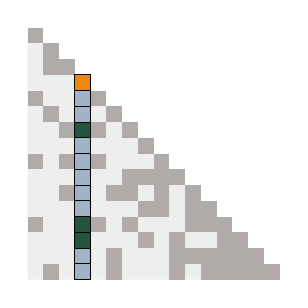
\begin{tikzpicture}[scale=1/5]
            % outer triangular factor
\fill[lightsilver] (0, 0) -- (0, -16) -- (16, -16) -- cycle;

% column rectangle
\draw[fill=lightblue] (3, -4) rectangle (4, -16);

% triangular factor
\fill[silver] (0, 0) rectangle (1, -1);
\fill[silver] (1, -1) rectangle (2, -2);
\fill[silver] (1, -2) rectangle (2, -3);
\fill[silver] (2, -2) rectangle (3, -3);
\fill[orange] (3, -3) rectangle (4, -4);
\draw (3, -3) rectangle (4, -4);
\fill[silver] (0, -4) rectangle (1, -5);
\draw (3, -4) rectangle (4, -5);
\fill[silver] (4, -4) rectangle (5, -5);
\fill[silver] (1, -5) rectangle (2, -6);
\draw (3, -5) rectangle (4, -6);
\fill[silver] (5, -5) rectangle (6, -6);
\fill[silver] (2, -6) rectangle (3, -7);
\fill[seagreen] (3, -6) rectangle (4, -7);
\draw (3, -6) rectangle (4, -7);
\fill[silver] (4, -6) rectangle (5, -7);
\fill[silver] (6, -6) rectangle (7, -7);
\draw (3, -7) rectangle (4, -8);
\fill[silver] (7, -7) rectangle (8, -8);
\fill[silver] (0, -8) rectangle (1, -9);
\fill[silver] (2, -8) rectangle (3, -9);
\draw (3, -8) rectangle (4, -9);
\fill[silver] (4, -8) rectangle (5, -9);
\fill[silver] (8, -8) rectangle (9, -9);
\draw (3, -9) rectangle (4, -10);
\fill[silver] (6, -9) rectangle (7, -10);
\fill[silver] (7, -9) rectangle (8, -10);
\fill[silver] (8, -9) rectangle (9, -10);
\fill[silver] (9, -9) rectangle (10, -10);
\fill[silver] (2, -10) rectangle (3, -11);
\draw (3, -10) rectangle (4, -11);
\fill[silver] (5, -10) rectangle (6, -11);
\fill[silver] (6, -10) rectangle (7, -11);
\fill[silver] (8, -10) rectangle (9, -11);
\fill[silver] (10, -10) rectangle (11, -11);
\draw (3, -11) rectangle (4, -12);
\fill[silver] (7, -11) rectangle (8, -12);
\fill[silver] (8, -11) rectangle (9, -12);
\fill[silver] (10, -11) rectangle (11, -12);
\fill[silver] (11, -11) rectangle (12, -12);
\fill[silver] (0, -12) rectangle (1, -13);
\fill[seagreen] (3, -12) rectangle (4, -13);
\draw (3, -12) rectangle (4, -13);
\fill[silver] (4, -12) rectangle (5, -13);
\fill[silver] (6, -12) rectangle (7, -13);
\fill[silver] (10, -12) rectangle (11, -13);
\fill[silver] (11, -12) rectangle (12, -13);
\fill[silver] (12, -12) rectangle (13, -13);
\fill[seagreen] (3, -13) rectangle (4, -14);
\draw (3, -13) rectangle (4, -14);
\fill[silver] (7, -13) rectangle (8, -14);
\fill[silver] (9, -13) rectangle (10, -14);
\fill[silver] (12, -13) rectangle (13, -14);
\fill[silver] (13, -13) rectangle (14, -14);
\draw (3, -14) rectangle (4, -15);
\fill[silver] (5, -14) rectangle (6, -15);
\fill[silver] (9, -14) rectangle (10, -15);
\fill[silver] (10, -14) rectangle (11, -15);
\fill[silver] (11, -14) rectangle (12, -15);
\fill[silver] (12, -14) rectangle (13, -15);
\fill[silver] (13, -14) rectangle (14, -15);
\fill[silver] (14, -14) rectangle (15, -15);
\fill[silver] (1, -15) rectangle (2, -16);
\draw (3, -15) rectangle (4, -16);
\fill[silver] (5, -15) rectangle (6, -16);
\fill[silver] (9, -15) rectangle (10, -16);
\fill[silver] (11, -15) rectangle (12, -16);
\fill[silver] (12, -15) rectangle (13, -16);
\fill[silver] (13, -15) rectangle (14, -16);
\fill[silver] (14, -15) rectangle (15, -16);
\fill[silver] (15, -15) rectangle (16, -16);

% column rectangle
\draw (3, -4) rectangle (4, -16);

          \end{tikzpicture}
        \end{subfigure}
        \begin{subfigure}[h]{0.4 \textwidth}
          \begin{tikzpicture}[overlay,remember picture]
            \node[below left=1.25cm and 1cm] at (current page.north east) {
                \includegraphics[width=2cm]{graphs/predict_cknn_2}
            };
          \end{tikzpicture}
        \end{subfigure}
    \end{figure}

    \vspace{-0.5cm}

    \begin{figure}[h!]
      \centering
      \includegraphics[width=\textwidth]{data/rho_kl-div}
    \end{figure}
  \end{column}
\end{columns}

% https://tex.stackexchange.com/questions/340058/uncovered-footnote-appears-too-early-in-beamer-presentation
\alt<3->{\footnotetext{\fullcite{schafer2020sparse}}}
{\let\thefootnote\relax\footnotetext{~ \newline ~}}
\end{frame}
\endgroup

\end{document}
